\subsection{Manipulationsknoten}

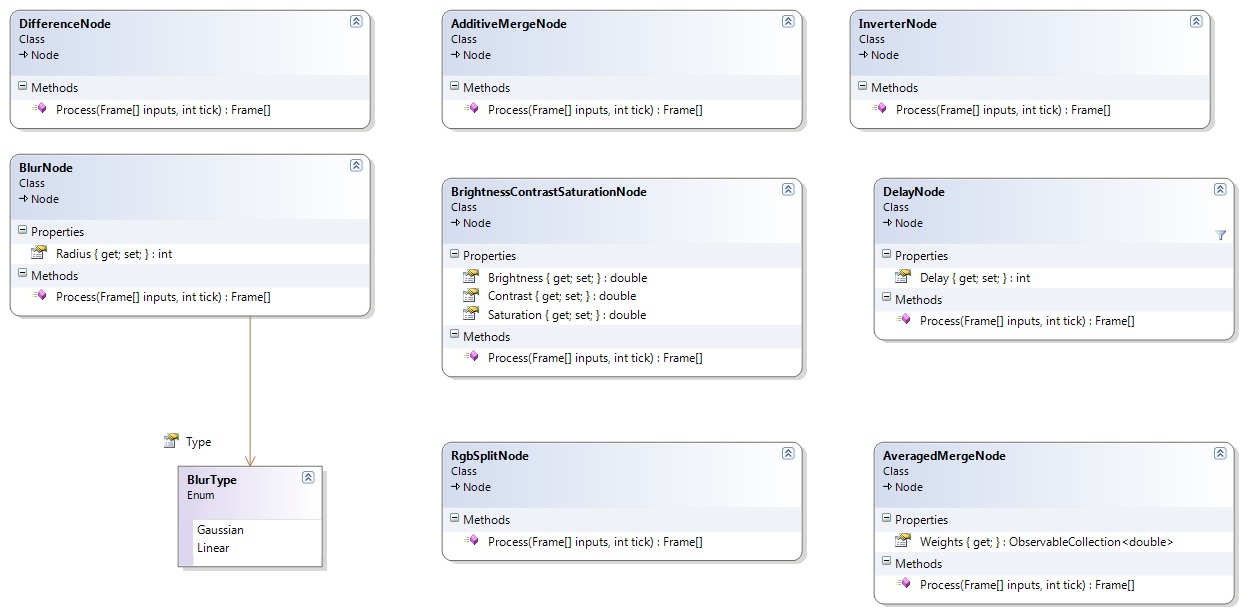
\includegraphics[width=\textwidth]{YuvKA.Pipeline/manipulationnodes.png}
for each manipulationnode do\\
this.mention

\subsubsection{YuvKA.Pipeline.InverterNode}

\subsubsection{YuvKA.Pipeline.BlurNode}

\subsubsection{YuvKA.Pipeline.BrightnessContrastSaturationNode}

\subsubsection{YuvKA.Pipeline.AdditiveMergeNode}

\subsubsection{YuvKA.Pipeline.AverageMergeNode}

\subsubsection{YuvKA.Pipeline.DifferenceNode}

\subsubsection{YuvKA.Pipeline.DelayNode}

\begin{verbatim}
public class DelayNode : Node
\end{verbatim}

\paragraph{Beschreibung}-\\
Die Klasse \name{DelayNode} modelliert die Verzögerung von Videostreams innerhalb der Pipeline.

\paragraph{Typmember}
\begin{itemize}

\field{Queue}
	\begin{verbatim}
	Queue<Frame> queue
	\end{verbatim}
	Enthält eine Warteschlange von \name{Frame}s die Verzögert werden.
	
\property{Delay}
	\begin{verbatim}
	[Range(0, 10)]
	public int Delay { get; set; }
	\end{verbatim}
	Ruft die Dauer der Verögerung in der Einheit \name{Frame}s ab, oder legt sie fest.

\method{ProcessFrame}
	\begin{verbatim}
	public override Frame[] ProcessFrame(Frame[] inputs, int frameIndex)
	\end{verbatim}
	Stellt die übergebenen \name{Frame}s in die die Warteschlange \name{Queue} mit der Länge \name{Delay} an, und gibt die ersten \name{Frame}s der Warteschlange zurück.
	
\end{itemize}

\subsubsection{YuvKA.Pipeline.RgbSplitNode}

